\chapter{Koncepcja i projekt systemu}
\label{cha:konception}

W niniejszy rozdział skupia się na przygotowaniu systemu do jego implementacji. Przedstawione zostały: w pierwszej sekcji ogólny opis systemu, następnie specyfikacja wymagań, w dalszej części architektura systemu, a na końcu projekt bazy danych.

\section{Ogólny opis systemu}

\subsection{Cele}
Głównym celem postawionym przed aplikacją internetową jest zapewnienie bezpieczeństwa na drodze, przy równoczesnym zachowaniu optymalnej przepustowości. Dlatego jej kluczowym elementem jest duża, czytelna mapa, na której umieszczone zostały dopuszczalne prędkości w zależności od różnych czynników drogowych, od typu nawierzchni, rodzaju drogi, ilości pasów ruchu, aż po pobliże budynków, przejść dla pieszych, sygnalizacji świetlnej czy przejazdów kolejowych. 

\subsection{Udziałowcy i użytkownicy}
\begin{itemize}
\item Użytkownicy aplikacji
\item Administratorzy
\end{itemize}

\subsection{Granice systemu (wejścia, wyjścia)}

\begin{figure}[h]
\caption{Granice systemu}
\label{sec:inOutBorder}
\centering
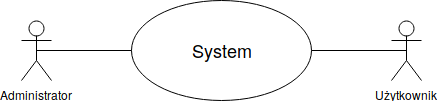
\includegraphics[width=0.8\textwidth]{inOutBorder}
\end{figure}

\newpage
\subsection{Podstawowe cele udziałowców i użytkowników}

\begin{table}[ht]
\centering
\caption{Podstawowe cele udziałowców i użytkowników}
\label{predkosciPromienKrzywizny2}
\begin{tabular}{| l | l | l | }
\hline
\textbf{Udziałowiec} & \textbf{Cel} & \textbf{Priorytet} \\ \hline
Administrator & Dodawanie domyślnych obiektów drogowych możliwych do wybrania & Wysoki\\ \hline
Administrator & Usuwanie domyślnych obiektów drogowych & Wysoki\\ \hline
Użytkownik & Wybieranie obiektów reprezentowanych przez punkt do mapy & Wysoki\\ \hline
Użytkownik & Wybieranie obiektów reprezentowanych przez dwuwymiarowe figury geometryczne & Wysoki\\ \hline
Użytkownik & Usuwanie obiektów reprezentowanych przez punkt do mapy & Wysoki\\ \hline
Użytkownik & Usuwanie obiektów reprezentowanych przez dwuwymiarowe figury geometryczne & Wysoki\\ \hline
Użytkownik & Wybieranie warstw mapy & Średni\\ \hline
Użytkownik & Wyświetlanie współrzędnych punktu & Niski \\ \hline
\end{tabular}
\end{table}


\subsection{Lista możliwości}
\begin{itemize}
\item Wyświetlanie mapy
\item Wyświetlanie warstw mapy w zależności od danego czynnika
\item Wyświetlanie współrzędnych obiektu
\item Dodawanie obiektów reprezentowanych przez punkt 
\item Dodawanie obiektów reprezentowanych przez dwuwymiarowe figury geometryczne
\item Usuwanie obiektów reprezentowanych przez punkt 
\item Usuwanie obiektów reprezentowanych przez dwuwymiarowe figury geometryczne
\end{itemize}

\newpage
\subsection{Diagram klas}

\begin{figure}[h]
\caption{Diagram klas}
\label{sec:inOutBorder}
\centering
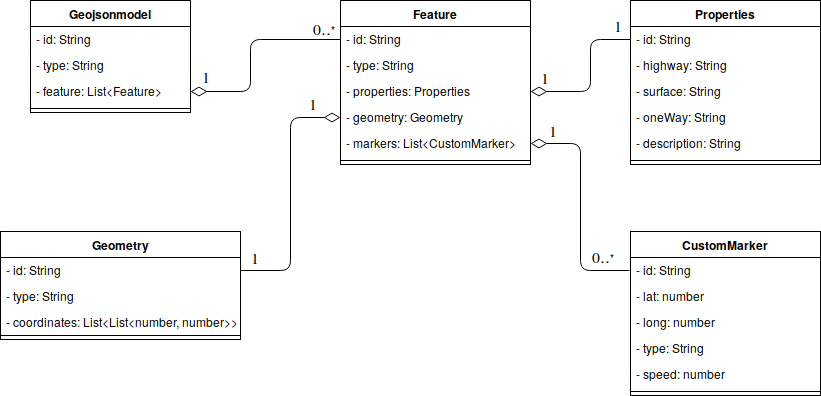
\includegraphics[width=1.05\textwidth]{diagramKlas}
\end{figure}

\section{Opis klas aplikacji}

Klasy aplikacji zostały podzielone na sześć grup:
\begin{itemize}
\item calcucationOperations
\item components
\item layerManagers
\item mapObjects
\item models
\item services
\end{itemize}
W niniejszej sekcji każde nich zostały dokładnie omówione

\newpage
\subsection{CalculationOperations}
W pakiecie calcutaionOperations znajdują się klasy odpowiedzialne za wykonywanie obliczanie dla poszczególnych części algorytmu. Składa się z:
\begin{itemize}
\item BoundingBox - klasa zajmująca się obliczeniami związanymi z minimalnym obszarem pokrywającym, dokładniej opisanym w rozdziale \ref{sec:Wyznaczanieminimalnegoobszarupokrywającego}, \ref{sec:Powiększanie wyznaczonegoobszarupokrywającego} oraz \ref{sec:laczeniepowiekszonychobszarwwpokrywajacych}
\item Curves - klasa zajmująca się obliczeniami związanymi z zakrętami. Opis znajduje się w rozdziale: \ref{sec:WyznaczaniePromieniaSkrętuDlaZakrętówDanejDrogi}
\end{itemize} 

\subsection{components}
W tym pakiecie znajdują się elementy odpowiedzialne za wyświetlanie danych oraz za sam wygląd strony. W skład nich wchodzą:
\begin{itemize}
\item app.component.ts - zajmuje się dostarczeniem danych do wyświetlenia
\item app.component.html - wyświetla dane na stronie
\item app.component.css - modyfikuje wygląd strony
\end{itemize}
\subsection{layerManagers}
Pakiet, w którym znajdują się klasy odpowiedzialne za przygotowanie warst mapy. Zostały w nim umieszczone:
\begin{enumerate}
\item BaseLayerManager - menadżer warstwy podstawowej
\item DbLayerManager - menadżer warstw wyświetlających przetworzone dane z bazy
\end{enumerate}
\subsection{mapObjects}
W tym pakiecie zostały umieszczone klasy odpowiedzialne za przetwarzanie obiektów. Należą do nich
\begin{itemize}
\item OneDimensions - klasa odpowiedzialna za przetwarzanie obiektów jednowymiarowych takich jak przejścia dla pieszych, przejazdy kolejowe oraz sygnalizacje świetlną
\item TwoDimension - klasa odpowiedzialna za przetwarzanie obiektów dwuwymiarowych takich jak szkoły, place zabaw, kościoły, sklepy, przystanki autobusowe i tramwajowe
\item OtherObjects - klasa odpowiedzialna za uzględnianie innych czynników znajdujących się na drodze, takich jak liczba pasów ruchu czy typ drogi.
\end{itemize}
\subsection{models}
\subsection{services}

\section{Architektura systemu}

System powstał na bazie stosu technologicznego MEAN Stack. Poniżej, na rys. \ref{sec:meanStackArchitecture} została przedstawiona architektura tego stosu.

\begin{figure}[h]
\caption{Architektura stosu MEAN}
\label{sec:meanStackArchitecture}
\centering
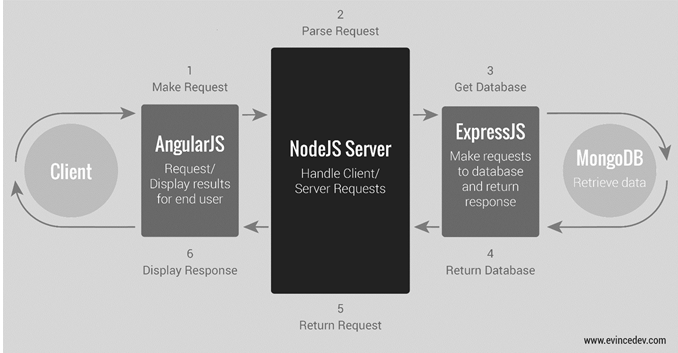
\includegraphics[width=0.83\textwidth]{meanArchitecture}
\source{Na podstawie evincedev.com}
\end{figure}

\newpage
Na rys. \ref{sec:meanStackArchitecture} został przedstawiony przebieg od wysłanego zapytania przez klienta do wyświetlonej odpowiedzi:  
\begin{enumerate}
\item Gdy klient wysyła zapytanie, najpierw jest ono przetwarzane przez Angulara po stronie klienta
\item W dalszej kolejności zapytanie zostaje przekazany do NodeJS po stronie serwera
\item Następnie zapytanie wędruje do ExpressJS, który pobiera dane z MongoDB.
\item Pobrane dane zostają z MongoDB zostają przekazane do ExpressJS
\item ExpressJS przesyła odpowiedź do Angulara
\item Angular wyświetla odpowiedź.
\end{enumerate}
